\section{Resistance, Resistivity, and Ideal Meters and Batteries}

\instructornote{%
By Matt, added to manual Fall 2020.  Time: ($\sim$ 20 minutes)

This is kind of a grab bag of exercises I've been doing in my classes for a while and am just now adding to the manual.  There's nothing Earth-shattering here, but these exercises are useful practice for students, and a good way to introduce the idea of real vs. ideal meters, real vs. ideal batteries, and also nice connections between resistivity and resistors in series and parallel.
}

\makelabheader %(Space for student name, etc., defined in master.tex)

\medskip
\textbf{Objectives}

\begin{itemize}[nosep]
\item Connect the idea of resistivity to resistors in series and parallel
\item Understand real vs. ideal voltmeters, ammeters, and batteries
\end{itemize}

\medskip
\textbf{Apparatus}

\begin{itemize}[nosep]
\item 2 digital multimeters 
\item 2 banana jumper wires
\end{itemize}

\medskip
\textbf{Activity 1: Resistivity, and Resistors in Series and Parallel}

\begin{enumerate}[labparts]

\item Suppose you have two ``resistors'' in series, which are both cylinders made of a material with resistivity $\rho$.  They have the same cross sectional area $A$, but different lengths $\ell_1$ and $\ell_2$.  Write their resistances below.

\begin{center}
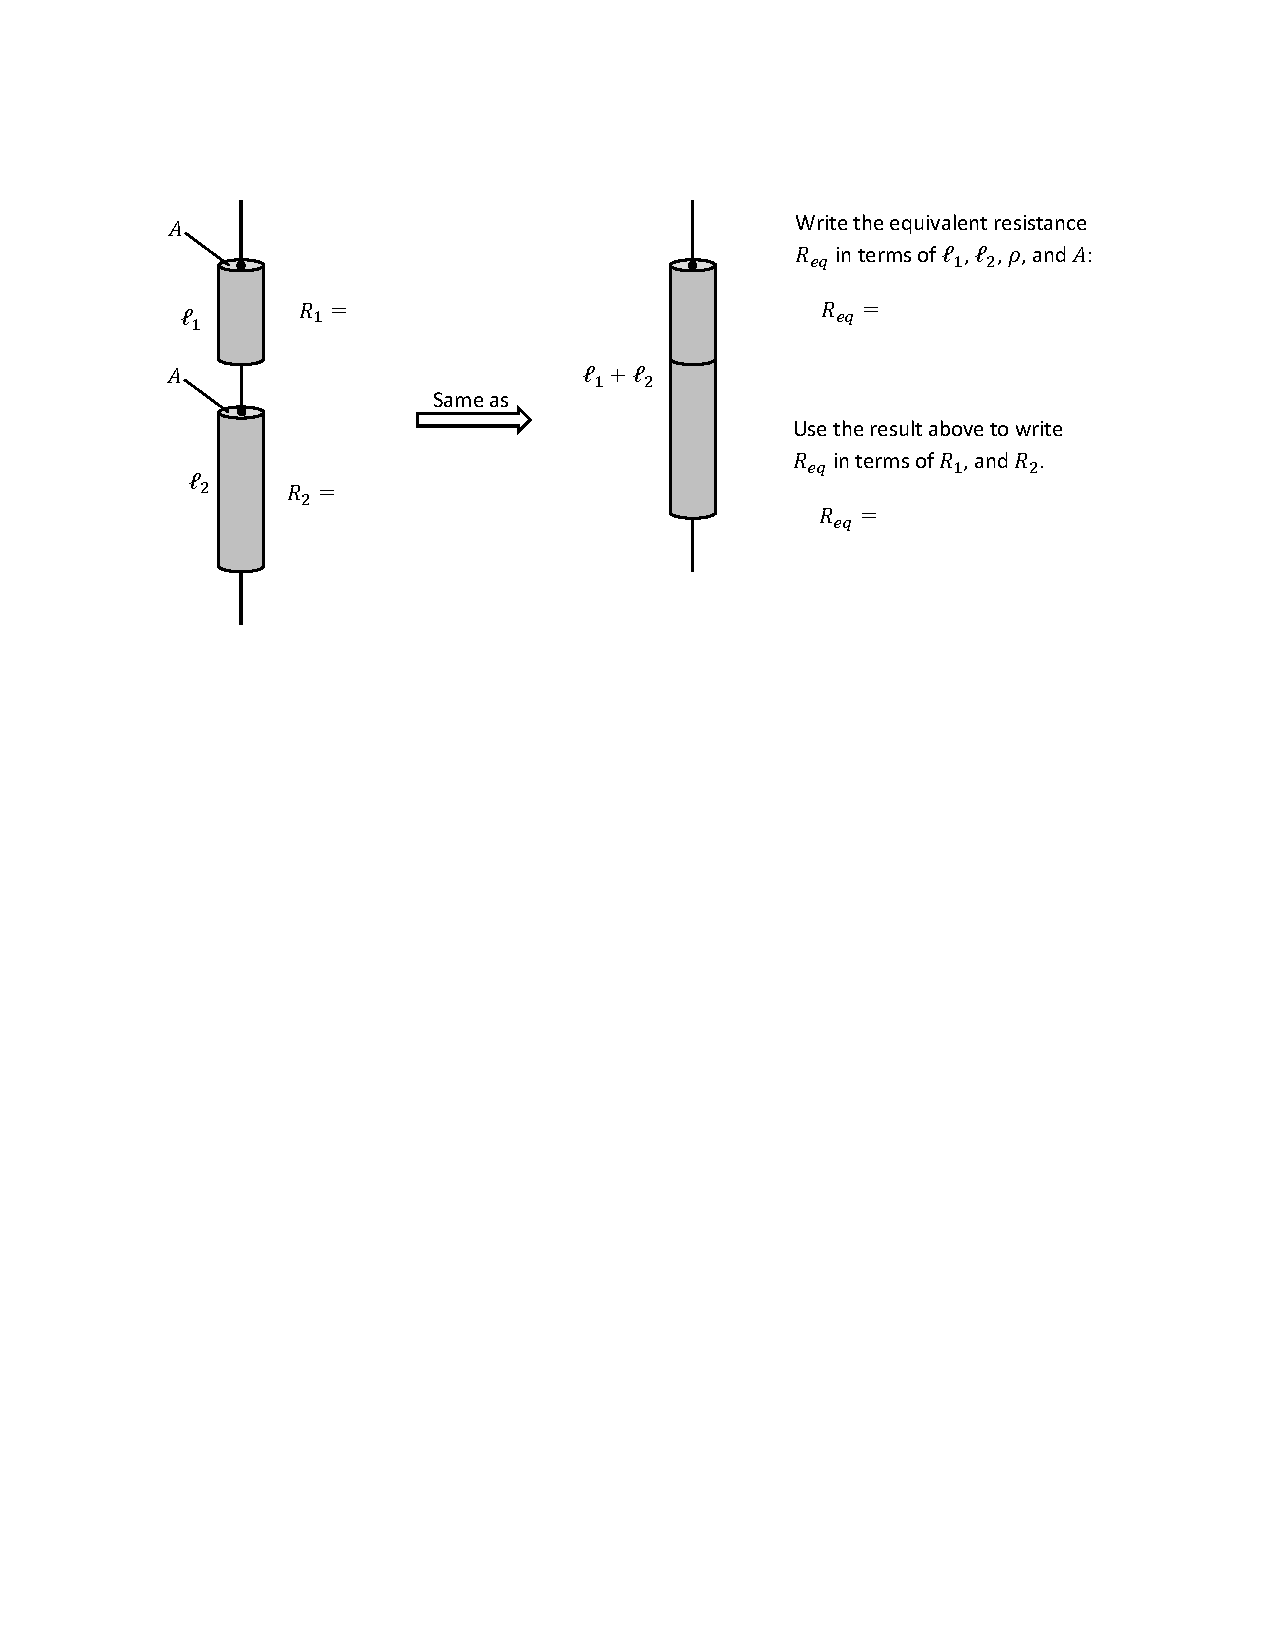
\includegraphics[scale=0.95]{resistance_ideal_meters/series_resistors.pdf}
\end{center}

\item Suppose you have two ``resistors'' in parallel, which are again both cylinders of the same material with resistivity $\rho$.  This time they have the same length $\ell$ but different cross-sectional areas $A_1$ and $A_2$.  Write their resistances below. 
\begin{center}
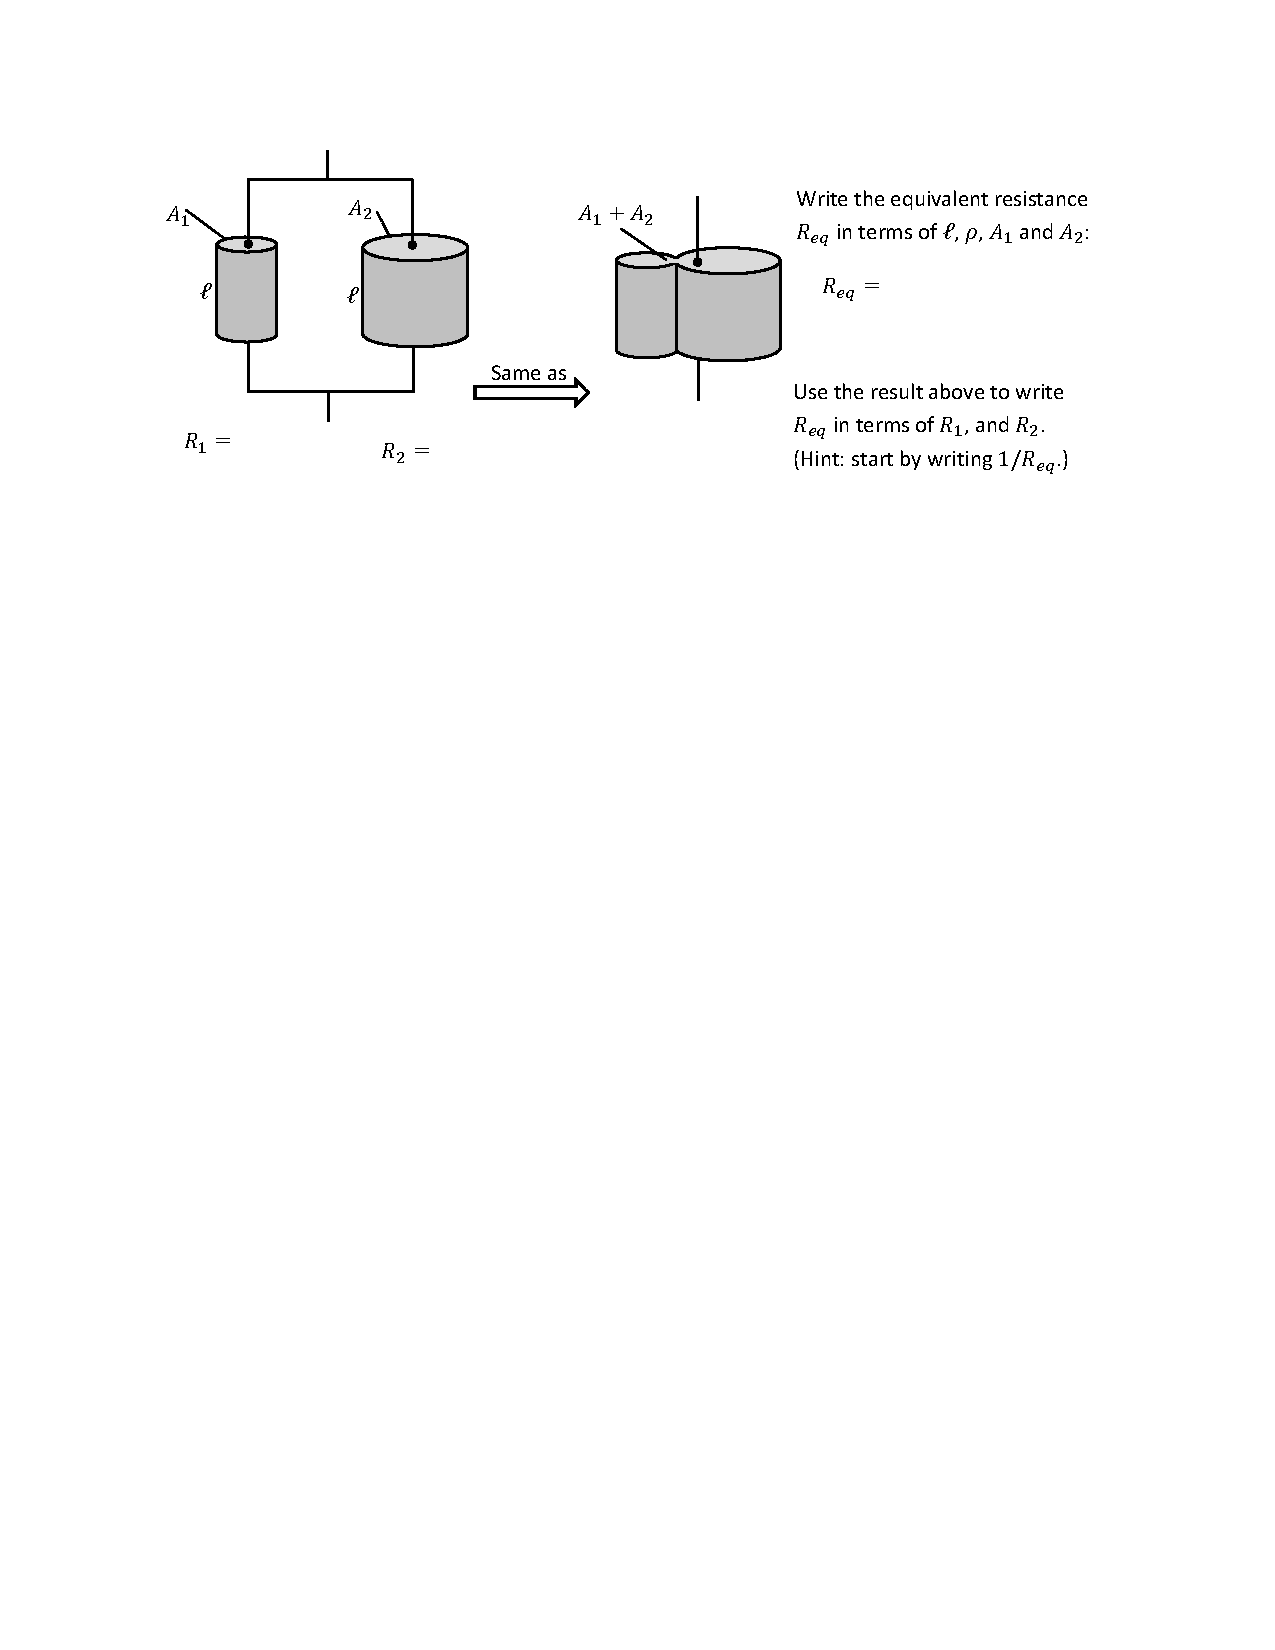
\includegraphics[scale=0.95]{resistance_ideal_meters/parallel_resistors.pdf}
\end{center}

\end{enumerate}
 
\textbf{Activity 2: Resistance of Ammeters and Voltmeters (Real and Ideal)}
 
 The circuit diagram below shows a battery connected to three light bulbs.

\bigskip

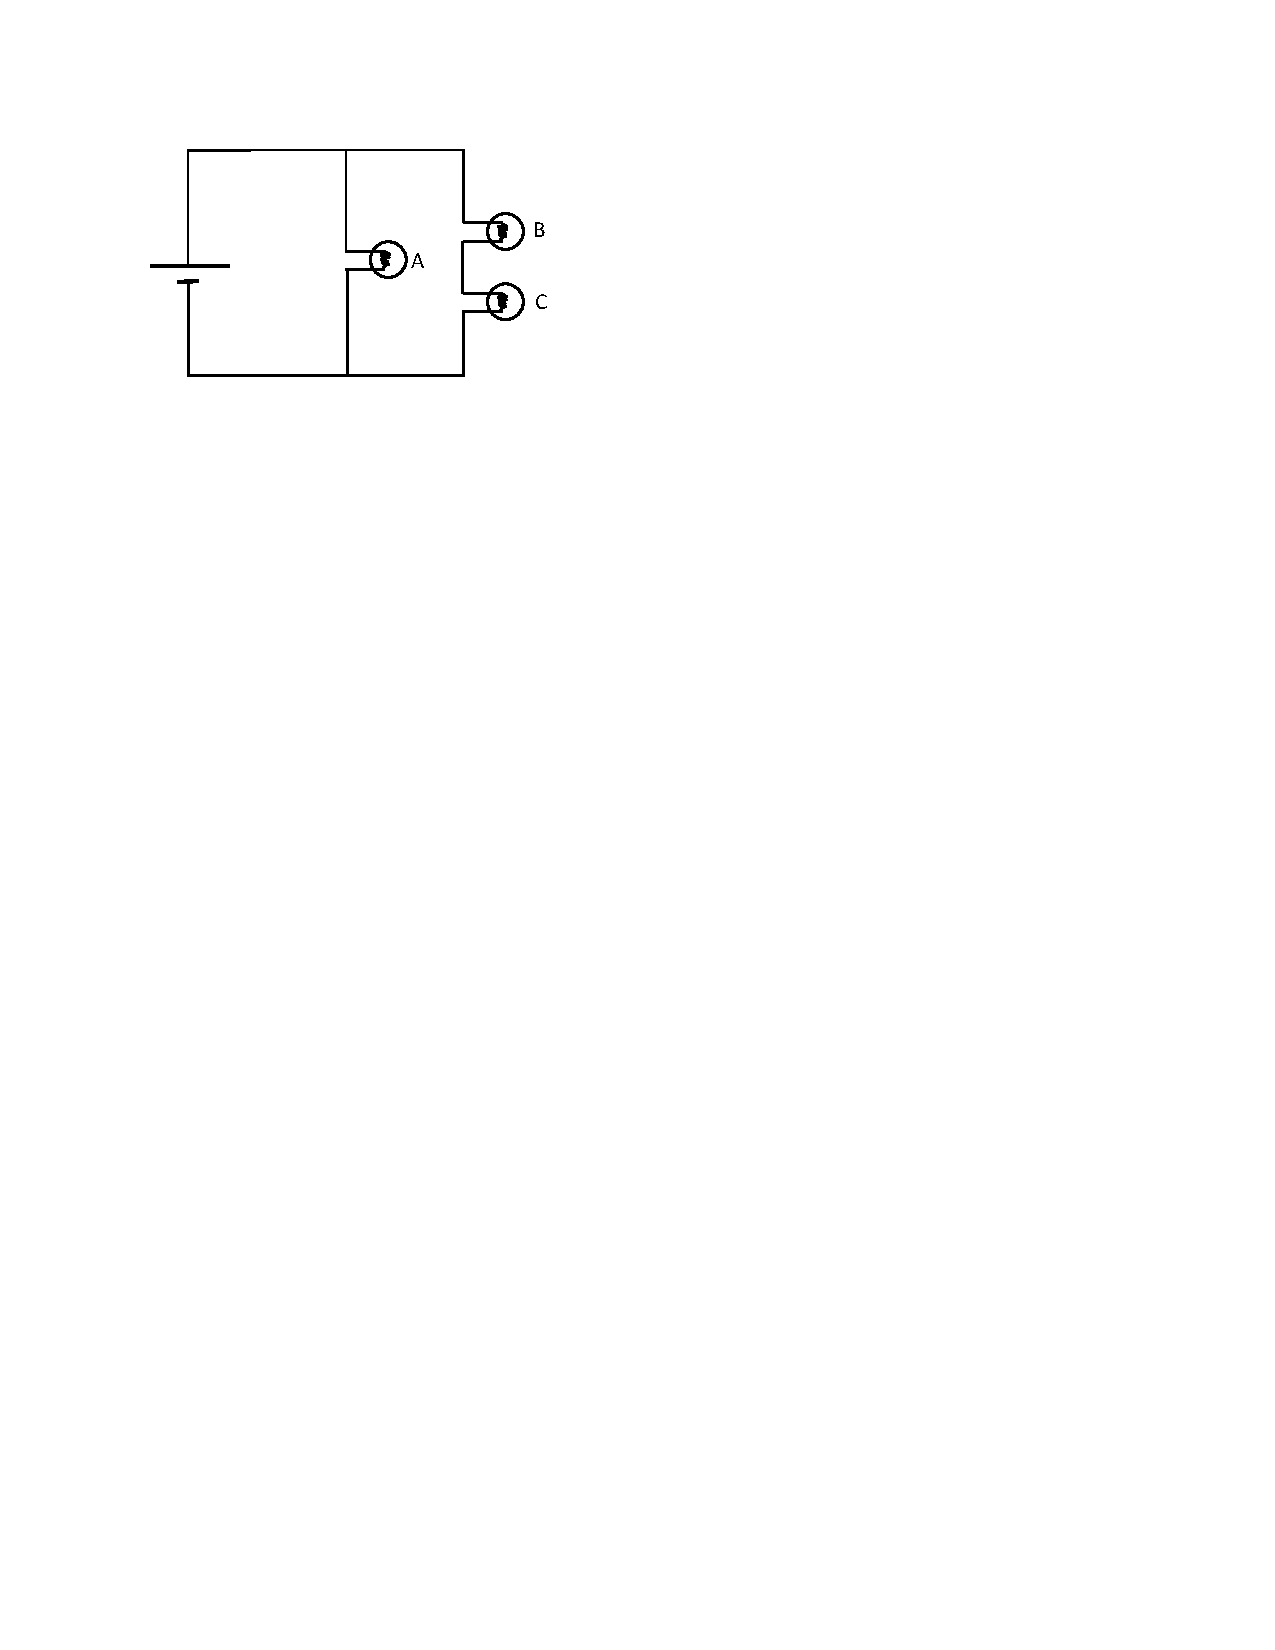
\includegraphics{resistance_ideal_meters/three_bulbs.pdf}

\answerspace{0.5in}

\begin{enumerate}[labparts]
 
\item In the space above, redraw the diagram to show how to add a current meter and a voltmeter to measure the current through bulb A, and the voltage across bulb C.

\item In general, you hope that when you connect current and voltage meters, they don't actually change any currents or voltages in your circuit.  Ideally, would you want the resistance of your current meter to be very small, very large, or somewhere in the middle?

\answerspace{0.5in}

\item You have two DMMs at your station.  Use one of them as a resistance meter (on ``$\Omega$'') to measure the resistance of the other meter when it is used as an ammeter.  Write your results below, for all possible current ranges on your meter (probably $\approx$20~A, $\approx$40~mA, etc.).  Was your prediction correct?

\answerspace{0.9in}

\item Ideally, would you want the resistance of your voltmeter to be very small, very large, or somewhere in the middle?

\answerspace{0.5in}

\item Use one of your meters to measure the resistance of the other meter when it is used as an voltmeter.  (It's possible that you won't be able to measure a value, but you can still confirm whether the resistance is high or low.)  Was your prediction correct?

\answerspace{0.9in}

\end{enumerate}

\pagebreak[3]

\textbf{Activity 3: Internal Resistance of a Battery}

An \textit{ideal} battery would always produce a constant emf $\mathcal{E}$ across a ``load'' resistance.  (The ``load'' means something useful like a motor or a light bulb.)  

\begin{enumerate}[labparts]
\item What would be the current $I$ through a load resistance of $R_{\rm load}=10~\Omega$, in the case of the \textit{ideal} battery below, with $\mathcal{E}=1.5$~Volts?

\bigskip
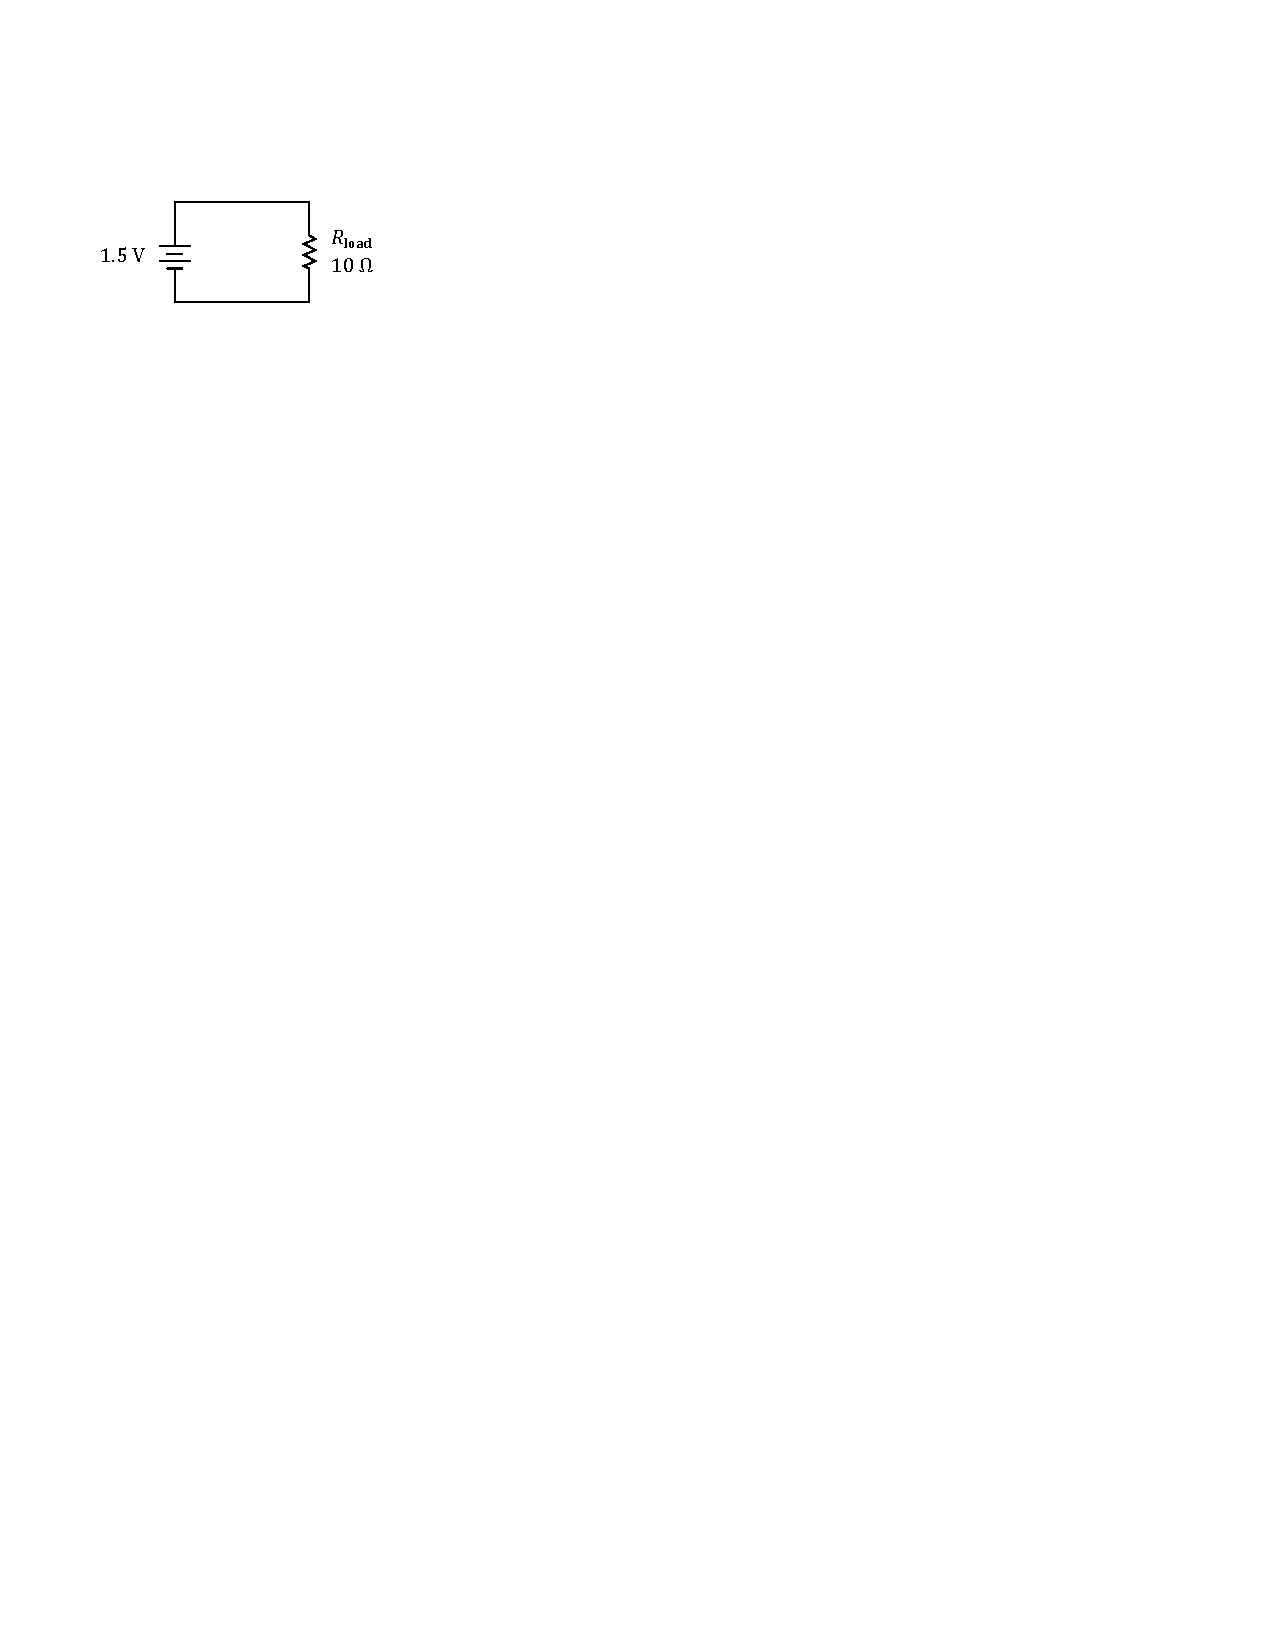
\includegraphics{resistance_ideal_meters/ideal_battery.pdf}
\bigskip

\item A \textit{real} (non-ideal) battery has an additional ``internal'' resistance $R_{\rm int}$ in series with its ideal source of emf~$\mathcal{E}$, as shown below.  For a typical 1.5 volt alkaline battery, $R_{\rm int}\approx 1~\Omega$.  What would be the current $I$ through a $10~\Omega$ load resistance in that case?

\bigskip
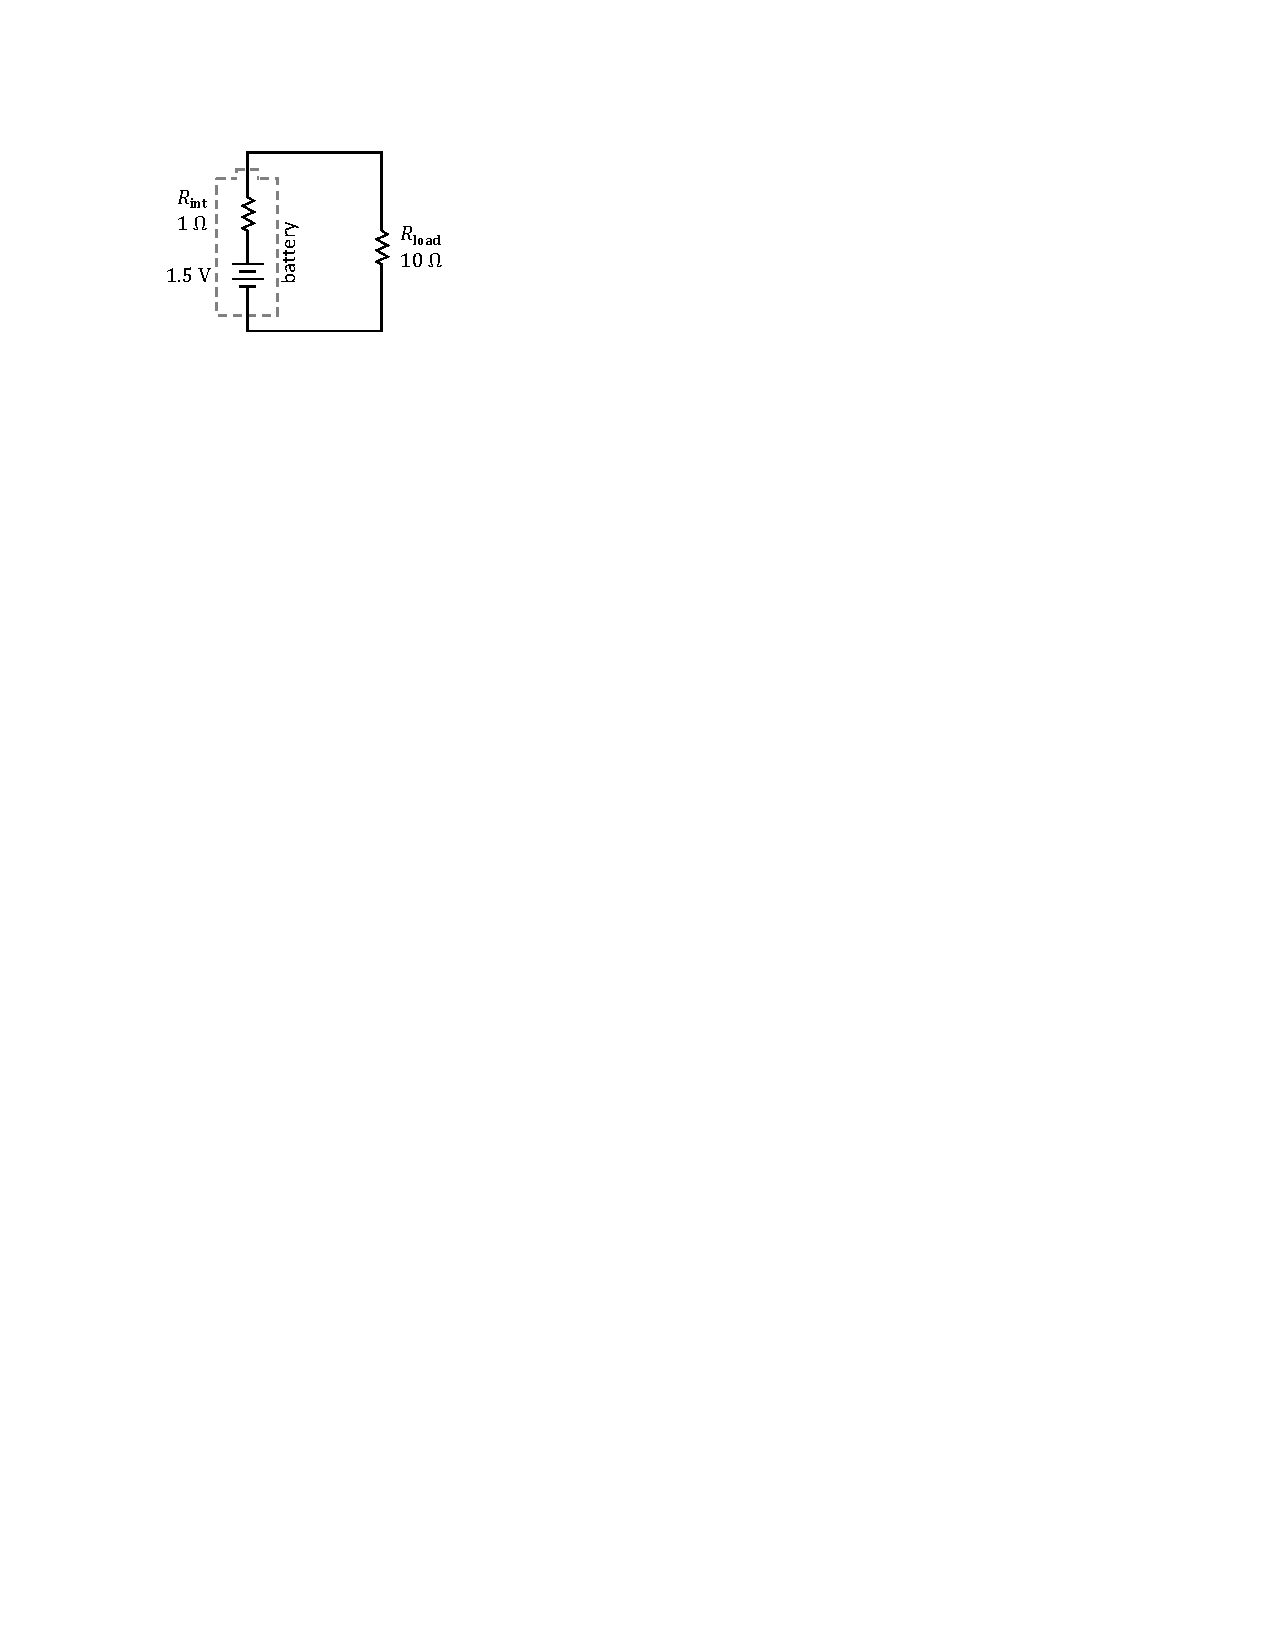
\includegraphics{resistance_ideal_meters/real_battery.pdf}
\answerspace{0.9in}

\item For the non-ideal battery above, with $\mathcal{E}=1.5$~volts and $R_{\rm int}=1~\Omega$, what would be the actual voltage across the $10~\Omega$ load resistance?
\answerspace{0.9in}

\item What current would the non-ideal battery above produce if you short-circuited the two terminals together?  (That is, if you replaced the load resistance with just a wire?)  
\answerspace{0.9in}

\item What would be the short-circuit current of an ``ideal'' battery?  Is that plausible?
\answerspace{0.9in}

\end{enumerate}



